% =====================================================================
%  Scale-Aware Joint Compression -- Results, Discussion, Limitations, Conclusion
%
%  Required preamble packages:
%    \usepackage{booktabs, amsmath, amssymb, algorithm, algpseudocode}
%    \usepackage{multirow, siunitx, pgfplots}  \pgfplotsset{compat=1.18}
%
%  All numbers below are regenerable:
%    python scripts/audit_confirmatory_run.py   # gate: must print AUDIT PASSED
%    python scripts/report_confirmatory.py      # T1--T5
%    python scripts/report_diagnostics.py       # mechanism tables
%    python scripts/build_paper_tables.py       # results/evidence/paper_tables.md
% =====================================================================

\section{Results}
\label{sec:results}

All results in \S\ref{subsec:headline}--\S\ref{subsec:qwen} are from a single frozen
execution on the held-out test split: $171$ records forming $42$ joint/sequential pairs,
zero failures, zero stale and zero missing records under the provenance gate of
\S\ref{subsec:stats}, on one host, at a single \texttt{method\_version}. Dense test
perplexities are $35.86$, $21.32$ and $17.26$ at 160M, 410M and 1B respectively.
Table~\ref{tab:budget} confirms that the realised budgets match across arms within every
cell, which is the precondition for reading any difference as a pipeline effect.

\begin{table}[t]
\centering
\caption{Budget realisation on the test split. All arms within a cell share mask sparsity,
effective bit width, module count and targeted-parameter count. Mask sparsity sits marginally
below $0.30$ because the per-row prune count is integral; effective bits exceed nominal width
by fp32 scale overhead, which shrinks with width as the group count per weight falls.
\textbf{Note the block counts:} pythia-1b is \emph{shallower} than pythia-410m, so the scale
axis is not monotone in depth (\S\ref{subsec:limits}).}
\label{tab:budget}
\small
\begin{tabular}{@{}lrrrrrr@{}}
\toprule
\textbf{Scale} & \textbf{Blocks} & \textbf{Modules} & \textbf{Targeted params} &
\textbf{Mask sparsity} & \textbf{Eff.\ bits W8} & \textbf{Eff.\ bits W4} \\
\midrule
pythia-160m & 12 & 48 & \num{84934656}  & 0.2997 & 8.0312 & 4.0312 \\
pythia-410m & 24 & 96 & \num{301989888} & 0.2999 & 8.0234 & 4.0234 \\
pythia-1b   & 16 & 64 & \num{805306368} & 0.2999 & 8.0117 & 4.0117 \\
\bottomrule
\end{tabular}
\end{table}

\subsection{Single-technique arms behave as expected}
\label{subsec:singletech}

Table~\ref{tab:retention} reports mean perplexity retention for every arm. The
single-technique arms are controls rather than competitors, and they establish that the
primitives behave sensibly before any joint claim is made. Quantisation alone at 8 bits is
essentially free ($99.85$--$99.96\%$ retention at every scale), confirming that W8 is a
near-inert precision. At 4 bits it costs $69.30\%$ / $64.38\%$ / $92.33\%$ retention at
160M / 410M / 1B --- and the ordering here is itself informative: the 1B model tolerates
4-bit quantisation far better than either smaller model, consistent with greater parameter
redundancy at scale. Pruning at $30\%$ is identical across budgets by construction, since
both budgets prune $30\%$ and differ only in precision.

\begin{table}[t]
\centering
\caption{Mean perplexity retention (\%) by arm, test split. Retention is
$100 \times \mathrm{PPL}_{\mathrm{dense}} / \mathrm{PPL}_{\mathrm{compressed}}$. Pruning and
quantisation are single-technique controls. The pruning column is constant within a scale
because both budgets prune $30\%$.}
\label{tab:retention}
\begin{tabular}{@{}llrrrr@{}}
\toprule
\textbf{Scale} & \textbf{Budget} & \textbf{Pruning} & \textbf{Quantisation} &
\textbf{Sequential} & \textbf{Joint} \\
\midrule
pythia-160m & 30\% + W8 & 79.75 & 99.95 & 79.72 & 79.76 \\
pythia-160m & 30\% + W4 & 79.75 & 69.30 & 55.81 & 56.82 \\
\midrule
pythia-410m & 30\% + W8 & 76.06 & 99.85 & 76.00 & 76.03 \\
pythia-410m & 30\% + W4 & 76.06 & 64.38 & 57.56 & 58.50 \\
\midrule
pythia-1b   & 30\% + W8 & 96.35 & 99.96 & 96.52 & 96.34 \\
pythia-1b   & 30\% + W4 & 96.35 & 92.33 & 89.65 & 89.79 \\
\bottomrule
\end{tabular}
\end{table}

\subsection{Implementation correctness anchors}
\label{subsec:anchors}

Because the effect under test is of order $\SI{1}{pp}$, an implementation fault could plausibly
produce or destroy it. We therefore validated the pipeline against three independent
references before interpreting any result, targeting the two halves of the method separately.

\paragraph{The mask is bit-identical to an independent implementation.} Our saliency rule is
the activation-weighted magnitude criterion, so an independent implementation given matched
inputs must produce the same mask. Compared across all $48$ targeted modules of Pythia-160M
--- \num{84934656} weights --- the masks agree in \textbf{zero differing positions}, with
worst per-module overlap $1.000000$ and column norms agreeing to $6.0 \times 10^{-7}$
relative. The two paths differ precisely where a fault would hide: ours derives
$\lVert X_{:,j}\rVert_2$ from the streamed Gram as $\sqrt{\operatorname{diag}(X^\top X)}$
while the reference sums column squares directly and never forms a Gram, so a streaming
fault cannot cancel; ours computes an exact prune count and scatters, while the reference
sorts and takes top-$k$ per row.

\paragraph{The solver never falls below the provable optimum.} For a fixed mask the objective
in \eqref{eq:gram} admits a closed-form per-row minimiser $\hat{w}_S = (H_{SS})^{-1}H_{S,:}w$.
Solving this exactly in float64 with no damping over $96$ rows (12 modules spanning four
module types and three depths) yields two hard invariants, both satisfied: \textbf{zero rows
score below the provable optimum} (required, since it is impossible) and \textbf{zero rows end
worse than naive masking} (required, since it is what the accept-only-if-better guard of
\eqref{eq:accept} exists to enforce). Mean improvement over naive masking is $+38.65\%$ of the
naive objective, at a mean efficiency of $0.6409$ of the achievable gain.

\paragraph{Absolute quality is credible against a published reference.} Internal consistency
does not establish that the numbers are in a plausible range. Compared against an unmodified
reference SparseGPT implementation at matched model, revision, calibration draw, module
coverage and evaluation loader --- the compression algorithm being the only unmatched
variable --- our pruning-only arm reaches $80.97\%$ retention against the reference's
$55.99\%$. We flag rather than celebrate this: a $\SI{24.98}{pp}$ advantage over a well-cited
reference is far more likely to indicate a misconfiguration than a genuine win, and it ran
opposite to our pre-recorded expectation. The gap is attributable to the mask comparison
group (per-output-row against tensor-wide) and to the criterion; matched on comparison group,
our arm sits within roughly $9\%$ relative perplexity of the canonical implementation.

\paragraph{Every implementation fault we found flattered the joint arm.} Six defects were
identified and corrected during development, and \emph{not one} ran in the other direction.
The most consequential were an objective mismatch in which each arm reconstructed against its
own intermediate rather than the dense weight, an unequal solver budget in which the joint arm
received twice the optimisation, and a baseline defect in which joint gain was measured
against $P{\to}Q$ alone where the protocol required best-of-both. This is simultaneously
reassuring and a reason for caution: the final estimate was reached by removing biases that
all pointed the same way, so it is conservative relative to the development-time figures ---
but the direction of historical error is itself grounds for scepticism about a sub-$\SI{1}{pp}$
positive result. The three anchors above bound what remains; bounding is not elimination.

\paragraph{Solver slack is bounded in sign but not in magnitude.} Arm-dependent solver
slack is real --- efficiency $0.6409$ under the sequential mask against $0.5631$ under the
joint mask --- but across $96$ exactly-solved rows it \textbf{never inverted which mask was
better}. The \emph{direction} of a measured joint gain is therefore not a solver artefact, and
the slack runs \emph{against} joint, understating rather than inflating it. The effect on
magnitude remains unquantified and cannot be closed by the same method: the exact minimiser
exists only for the continuous least-squares problem, and the discrete grid makes the
quantised version an integer program with no closed form.

\subsection{The confirmatory result: no cell is practically important}
\label{subsec:headline}

Table~\ref{tab:main} is the study's primary result. Under the pre-registered criterion of
\S\ref{subsec:stats} --- mean gain $\geq \SI{1.0}{pp}$ \emph{and} a consistent sign across
every paired replicate --- \textbf{no cell qualifies}.

\begin{table}[t]
\centering
\caption{Joint gain over the \emph{frozen} sequential baseline, test split. $\S$6.3 requires
mean gain $\geq \SI{1.0}{pp}$ \textbf{and} sign consistency across all replicates. No cell
meets both. Holm-adjusted $p$-values correct for the six cells examined and are the values we
quote; raw values are shown only for transparency. The baseline is the order frozen per cell
on validation, not best-of-both, so the W8 rows carry an order uncertainty comparable in
magnitude to their effect.}
\label{tab:main}
\small
\begin{tabular}{@{}llcrrrcrrc@{}}
\toprule
\textbf{Scale} & \textbf{Budget} & \textbf{Order} & \textbf{R} &
\textbf{Mean (pp)} & \textbf{SD} & \textbf{Positive} &
\textbf{Raw $p$} & \textbf{Holm $p$} & \textbf{$\S$6.3} \\
\midrule
pythia-160m & 30\% + W8 & $P{\to}Q$ & 8 & $+0.0381$ & 0.0847 & 5/8 & 0.7266 & 1.0000 & no \\
pythia-160m & 30\% + W4 & $P{\to}Q$ & 8 & $\mathbf{+1.0120}$ & 0.7812 & 7/8 & 0.0703 & 0.3125 & no \\
pythia-410m & 30\% + W8 & $P{\to}Q$ & 8 & $+0.0289$ & 0.0521 & 5/8 & 0.7266 & 1.0000 & no \\
pythia-410m & 30\% + W4 & $P{\to}Q$ & 8 & $\mathbf{+0.9348}$ & 0.6233 & \textbf{8/8} & \textbf{0.0078} & \textbf{0.0469} & no \\
pythia-1b   & 30\% + W8 & $Q{\to}P$ & 5 & $\mathbf{-0.1794}$ & 0.0727 & \textbf{0/5} & 0.0625 & 0.3125 & no \\
pythia-1b   & 30\% + W4 & $P{\to}Q$ & 5 & $+0.1316$ & 0.1858 & 4/5 & 0.3750 & 1.0000 & no \\
\bottomrule
\end{tabular}
\end{table}

\paragraph{The two 4-bit cells fail on opposite criteria, each by a narrow margin.} At 160M
the mean gain clears the effect-size threshold ($+\SI{1.0120}{pp}$) but replicate 3 is
negative ($-\SI{0.3148}{pp}$), breaking sign consistency. At 410M the gain is unanimous
across all eight replicates --- the only cell in the study to reach significance --- yet
lands $\SI{0.065}{pp}$ short of the threshold. We record this explicitly because it is
precisely the configuration in which a pre-registered bar tends to be quietly renegotiated.
The threshold was fixed before any test-split data existed and we do not move it.

\paragraph{Significance requires correction, and barely survives it.} Six cells were
examined and the largest is being reported. Under Holm--Bonferroni correction the 410M
4-bit cell's raw $p = 0.0078$ becomes $p = 0.0469$: still below $0.05$, by $0.0031$. No other
cell survives correction; the next smallest adjusted value is $0.3125$. The same cell is thus
simultaneously marginally significant \emph{and} short of the practical bar. The defensible
summary is that this effect is real but small and fragile, not that it is established.

\paragraph{At 8 bits the mechanism produces nothing, and at 1B it is harmful.} The two
smaller-scale W8 cells carry small positive means but are not sign-consistent ($5/8$ each,
$p = 0.7266$), so they are indistinguishable from zero. The 1B W8 cell is different in kind:
all five replicates are negative and all five paired-bootstrap intervals exclude zero on the
negative side. This is a small but reliable \emph{disadvantage} for the joint arm --- the
mechanism does not merely fail to help at 8 bits at scale, it costs a fraction of a
percentage point.

\paragraph{Replicate-level spread justifies the design.} At 4-bit precision the
replicate-to-replicate standard deviation ($0.78$ and $0.62$ pp at 160M and 410M) is
comparable to the effect being measured. A single calibration draw at 160M could have
reported anywhere from $-\SI{0.31}{pp}$ to $+\SI{2.11}{pp}$. Any single-draw comparison at
this budget is therefore uninformative about the sign, which we take as the central
methodological lesson of the study.

\subsection{Neither exploratory estimate replicated}
\label{subsec:replication}

Before the confirmatory run, exploratory estimates on the validation split suggested a clean
monotone decline. Table~\ref{tab:replication} shows what happened when those cells were
re-measured on held-out data with more than double the replicates.

\begin{table}[t]
\centering
\caption{Exploratory (validation, $R{=}3$) against confirmatory (test, $R{=}8$ or $5$)
estimates at the aggressive budget. The two larger estimates moved \emph{toward} each other
--- the signature of regression from a selection surface.}
\label{tab:replication}
\begin{tabular}{@{}lllr@{}}
\toprule
\textbf{Cell} & \textbf{Exploratory} & \textbf{Confirmatory} & \textbf{Movement} \\
\midrule
160M, W4 & $+1.69$ pp, 3/3 & $+1.0120$ pp, 7/8 & $-0.68$ pp, unanimity lost \\
410M, W4 & $+0.39$ pp, 2/3 & $+0.9348$ pp, 8/8 & $+0.54$ pp, unanimity gained \\
1B, W4   & $+0.20$ pp, 3/3 & $+0.1316$ pp, 4/5 & held \\
\bottomrule
\end{tabular}
\end{table}

The 410M reversal is the most consequential: the scale point the exploratory work had written
off as null is the one cell that reaches significance. This is not a defect of the
exploratory phase but its intended function --- the validation split is a declared selection
surface, and estimates taken from a surface used for selection are expected to regress. We
report it prominently because it is the strongest available evidence that the two-split
design earned its cost, and because it means any published single-split result at this effect
size should be treated with caution.

\subsection{The scale trend, stated conservatively}
\label{subsec:trend}

\begin{table}[t]
\centering
\caption{Joint gain (pp) across scale and precision, test split. Every W4 cell is positive;
every W8 cell is near zero or negative. \textbf{Qwen2.5-0.5B is an external-validity check,
not a fourth scale point}, and must not be interpolated into the Pythia trend.}
\label{tab:trend}
\begin{tabular}{@{}lrrrcr@{}}
\toprule
\textbf{Budget} & \textbf{160M} & \textbf{410M} & \textbf{1B} & & \textbf{Qwen 0.5B} \\
\midrule
30\% + W4 & $+1.0120$ & $+0.9348$ & $+0.1316$ & & $+0.4213$ \\
30\% + W8 & $+0.0381$ & $+0.0289$ & $-0.1794$ & & $-0.0321$ \\
\bottomrule
\end{tabular}
\end{table}

\begin{figure}[t]
\centering
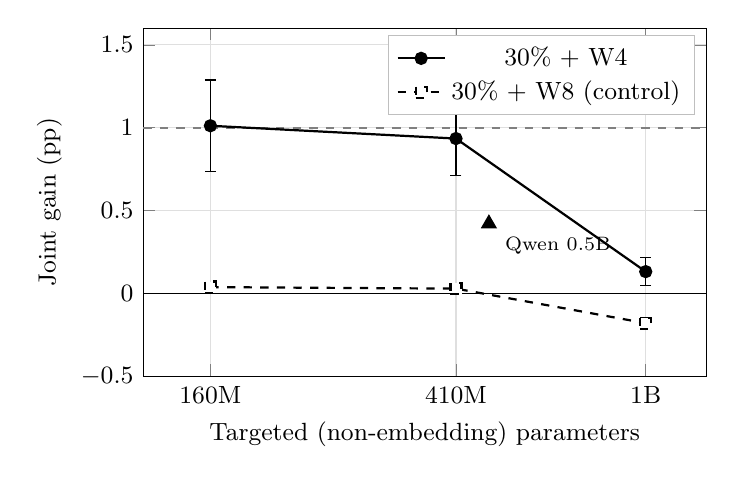
\begin{tikzpicture}
\begin{semilogxaxis}[
    width=0.72\textwidth, height=6cm,
    xlabel={Targeted (non-embedding) parameters},
    ylabel={Joint gain (pp)},
    xmin=6e7, xmax=1.1e9,
    ymin=-0.5, ymax=1.6,
    xtick={8.49e7, 3.02e8, 8.05e8},
    xticklabels={160M, 410M, 1B},
    grid=major, grid style={gray!25},
    legend style={at={(0.98,0.98)}, anchor=north east, font=\small, draw=gray!50},
    tick label style={font=\small}, label style={font=\small},
]
\addplot[dashed, gray, thick, forget plot] coordinates {(6e7,1.0) (1.1e9,1.0)};
\node[gray, font=\scriptsize, anchor=south east] at (axis cs:1.05e9,1.02) {practical bar (1.0 pp)};
\addplot[black, thick, mark=*, error bars/.cd, y dir=both, y explicit]
  coordinates {
    (8.49e7, 1.0120) +- (0, 0.2762)
    (3.02e8, 0.9348) +- (0, 0.2204)
    (8.05e8, 0.1316) +- (0, 0.0831)
  };
\addlegendentry{30\% + W4}
\addplot[black, thick, dashed, mark=square*, mark options={fill=white},
         error bars/.cd, y dir=both, y explicit]
  coordinates {
    (8.49e7, 0.0381) +- (0, 0.0299)
    (3.02e8, 0.0289) +- (0, 0.0184)
    (8.05e8, -0.1794) +- (0, 0.0325)
  };
\addlegendentry{30\% + W8 (control)}
\addplot[black, only marks, mark=triangle*, mark size=3pt, forget plot]
  coordinates {(3.58e8, 0.4213)};
\node[font=\scriptsize, anchor=north west] at (axis cs:3.7e8, 0.40) {Qwen 0.5B};
\addplot[black, thin, forget plot] coordinates {(6e7,0) (1.1e9,0)};
\end{semilogxaxis}
\end{tikzpicture}
\caption{Joint gain against targeted parameter count. Error bars are standard errors over
paired calibration replicates ($R{=}8$ at 160M and 410M, $R{=}5$ at 1B). The W4 gain is
positive at all three scales but does not increase with scale and never clears the
pre-registered $\SI{1.0}{pp}$ bar under both criteria; the W8 control sits at or below zero.
\textbf{Qwen2.5-0.5B (triangle) is plotted for reference only and is excluded from any
fit} --- it is a different model family, not a fourth scale point, and its horizontal
placement should not be read as interpolating the Pythia trend.}
\label{fig:trend}
\end{figure}

The motivating hypothesis --- that joint optimisation pays off \emph{more} at scale --- is
\textbf{not supported} (Figure~\ref{fig:trend}). The observed direction is the opposite, at
both budgets. Three considerations prevent us from stating this as a refutation:

\begin{enumerate}
  \item \textbf{The shape is not a monotone decline.} The 160M and 410M cells lie within
        $\SI{0.08}{pp}$ of one another; effectively all of the movement sits in the
        410M~$\rightarrow$~1B step. Two points at one level and a third below them is a
        weaker basis for a trend than three ordered points.
  \item \textbf{No test compares scales.} Every $p$-value reported here is within-cell.
        Differences \emph{between} cells carry no significance test, and with three points
        none is available.
  \item \textbf{The one large step is confounded with depth.} pythia-1b has 16 decoder
        blocks against pythia-410m's 24 (Table~\ref{tab:budget}). Since the method is
        layerwise and error compensation is applied block by block, the number of blocks is
        the number of opportunities for a joint step to help. The decline at 1B coincides
        with a decline in depth, and this design cannot separate them.
\end{enumerate}

The defensible claim is therefore: \emph{the joint advantage did not increase with scale, the
observed direction was opposite, and at no scale does it reach practical importance.}

\subsection{A fixed recipe does not imply matched effective severity}
\label{subsec:severity}

Before attributing the trend to scale, one confound must be made explicit, because it is a
genuine alternative explanation rather than a caveat. Both budgets prune $30\%$ at every
scale, which holds the \emph{recipe} constant. It does not hold the \emph{damage} constant.
Retention at the aggressive budget runs $55.81\%$ / $57.56\%$ / $89.65\%$ across
160M / 410M / 1B (Table~\ref{tab:retention}): the same recipe is far milder at 1B.

This matters directly for interpretation. A sequential baseline that already retains $89.65\%$
leaves little quality for a better layer solution to recover, so the same local mechanism buys
less end-to-end even if it is working exactly as well. ``Joint helps less at scale'' and
``joint helps less when there is less to recover'' are not distinguished by this design.
Nominal severity was matched across scales; \emph{effective} severity was not, and larger
models tolerating compression better is a robustness that benefited the sequential baseline
too.

We therefore do not claim that the three Pythia scales experienced equal effective severity,
and we treat headroom as a live competing explanation for the trend alongside the depth
confound of \S\ref{subsec:trend}.

\subsection{Mechanism: the local effect does not weaken, its translation does}
\label{subsec:mechanism}

Because the aggregate trend admits multiple readings, we instrumented the solver itself.
Table~\ref{tab:mechanism} reports three layer-level diagnostics computed from the committed
confirmatory records without re-running anything.

\begin{table}[t]
\centering
\caption{Layer-level mechanism diagnostics, test split. \emph{Mask divergence} is the
fraction of mask positions the joint refinement moves away from the sequential choice;
\emph{layer gain} and \emph{objective advantage} are computed on final layer losses, matched
layer by layer. At W4 every local quantity is at or above its 160M value at 1B, while
end-to-end gain falls by roughly $8\times$.}
\label{tab:mechanism}
\begin{tabular}{@{}lrrrrr@{}}
\toprule
& \multicolumn{2}{c}{\textbf{Mask divergence}} & \multicolumn{2}{c}{\textbf{Layer objective adv.}} & \textbf{End-to-end} \\
\cmidrule(lr){2-3}\cmidrule(lr){4-5}
\textbf{Scale} & \textbf{W8} & \textbf{W4} & \textbf{W8} & \textbf{W4} & \textbf{gain, W4 (pp)} \\
\midrule
pythia-160m & 0.0036\% & 3.6896\% & $+0.0039\%$ & $+2.1647\%$ & $+1.0120$ \\
pythia-410m & 0.0009\% & 2.9241\% & $-0.4911\%$ & $+2.2826\%$ & $+0.9348$ \\
pythia-1b   & 0.0019\% & 3.4063\% & $+0.1668\%$ & $+2.3214\%$ & $+0.1316$ \\
\bottomrule
\end{tabular}
\end{table}

Two findings follow.

\paragraph{The precision-specificity prediction is confirmed at every scale.} Mask divergence
differs by roughly three orders of magnitude between W8 and W4. This was predicted from the
method's construction (\S\ref{subsec:joint}) before the confirmatory data existed: at 8 bits
quantisation error is too small to reorder the saliency ranking, so the joint and sequential
masks nearly coincide and there is no mechanism to produce a difference. The W8 columns of
Table~\ref{tab:main} are the behavioural consequence. This is the one structural claim that
looks identical before and after the freeze.

\paragraph{The mechanism does not weaken with scale --- its translation into quality does.}
At W4, mask divergence at 1B ($3.41\%$) is comparable to 160M ($3.69\%$), and the local layer
objective advantage is in fact \emph{highest} at 1B ($+2.32\%$, with joint winning $317/320$
layers). Yet end-to-end gain falls from $+\SI{1.01}{pp}$ to $+\SI{0.13}{pp}$. The joint step
continues to find better local solutions at scale; those solutions stop translating into
model-level quality.

This is a dissociation, not an explanation, and our evidence does not close it. Two candidates
are consistent with the data and neither is tested here. \emph{Headroom}: the 1B aggressive
cell retains $89.65\%$ against 160M's $55.81\%$, so a baseline that already loses little
leaves little for a better layer solution to recover. \emph{Depth}: layerwise reconstruction
compounds through the compressed prefix, and 1B has fewer blocks than 410M. Distinguishing
them requires either a depth-matched pair or a scale point with different headroom at the
same depth, neither of which the Pythia suite provides.

\subsection{External validation in a second model family}
\label{subsec:qwen}

We repeated the protocol on Qwen2.5-0.5B ($65$ cells, $16/16$ pairs, $R{=}8$, test split,
single host). Qwen2 differs from Pythia in tokeniser, vocabulary ($\num{151936}$), training
corpus, attention configuration (grouped-query, 14 query heads to 2 key/value heads) and
embedding tying. Absolute perplexity is consequently incomparable with Pythia's; only
retention ratios and the sign of the effect transfer.

At the aggressive budget the gain is $+\SI{0.4213}{pp}$ ($7/8$ positive, raw $p = 0.0703$,
Holm $p = 0.1406$); at the moderate budget it is $-\SI{0.0321}{pp}$ ($1/8$ positive). Neither
cell meets the pre-registered criterion --- the W4 cell fails on \emph{both} counts, being
$\SI{0.58}{pp}$ short of the threshold and not sign-consistent --- and neither reaches
significance before or after correction.

What transfers is the \emph{structure}: W4 positive, W8 at or below zero, in a second family
with a different tokeniser and corpus (Table~\ref{tab:trend}). What does not transfer is any
claim of practical importance. We also note that the Qwen validation-split estimate
($+\SI{0.6216}{pp}$) again overstated its test-split value ($+\SI{0.4213}{pp}$) --- the third
independent instance in this study of a validation figure failing to hold on test.

\subsection{Downstream task accuracy}
\label{subsec:downstream}

Perplexity is not the only quality functional of interest, so we evaluated HellaSwag, PIQA
and ARC-Easy on full tasks with a pinned harness. Dense scores reproduce published Pythia
values to within $\SI{0.30}{pp}$ across nine cells, which is the anchor that makes anything
measured on top of them interpretable.

Compression costs measurable downstream accuracy: retention against each model's own dense
score ranges from $0.993$ (HellaSwag, 160M) down to $0.897$ (ARC-Easy, 410M), with ARC-Easy
consistently the most sensitive task. Every arm at every scale remains demonstrably above
chance.

\textbf{No joint-versus-sequential difference is resolvable on these tasks.} Across nine
model--task cells, not one difference reaches $1\sigma$ of its own standard error, let alone
$2\sigma$. This is a \emph{bounded} null rather than evidence of no effect: ARC-Easy at 160M
would require roughly four times the item count to resolve the $\SI{1.39}{pp}$ difference
observed, and these tasks are fixed-size.

We note one instructive tension. At 160M aggressive, perplexity favours joint while all three
downstream tasks place it marginally behind. Both can hold simultaneously: perplexity is
average log-likelihood over natural text, whereas multiple-choice accuracy is an argmax over
candidate continuations, and a method can lower average NLL while degrading the ranking
between a correct completion and a plausible distractor. Since every downstream difference
here is under $1\sigma$ on a single draw, we do not use either endpoint to argue against the
other.

\subsection{Deployment: sparsity does not become speed}
\label{subsec:latency}

Under the measurement protocol of \S\ref{subsec:deployment} --- CPU only, single host, pinned
threads, model-order rotation, 60 samples per cell --- we separate prefill from decode
latency. The prefill/decode structure behaves as theory requires at all three scales: for a
$4\times$ longer prompt, prefill scales by $3.79\times$ / $4.00\times$ / $3.98\times$ while
decode scales by only $1.36\times$ / $1.21\times$ / $1.22\times$. This compute-bound versus
bandwidth-bound distinction would have been concealed by a single blended generation latency,
and it doubles as an implementation check: had the decode callable silently re-run the
prompt, decode would have tracked prefill's $4\times$.

\textbf{$30\%$ unstructured sparsity delivers no commensurate speedup.} Against the dense
baseline, $9$ of $12$ cells lean faster by $1$--$3\%$, but $9/12$ reaches only $p = 0.15$ on
an exact sign test and every gap lies inside the interquartile range. Against what the
compression ratio would predict --- roughly $30\%$ if the pruned weights were being skipped
--- the measured $1$--$3\%$ is an order of magnitude short. The cause is mechanical: an
unstructured mask stores zeros, and a dense BLAS kernel multiplies by them rather than
skipping them.

\paragraph{This study contains no joint-versus-sequential latency comparison.} We state this
plainly because its absence is structural rather than incidental. Every packed arm ---
quantisation, sequential and joint, at both precisions --- is refused a latency measurement
by a runtime-representation gate, because a packed low-bit artefact would be timed through a
dequantising path and the resulting number would measure the unpacking kernel rather than
inference. Only the FP32 arms can be timed natively. The sparsity-to-speedup question is
therefore answerable only through the pruning-only arm, and the answer at $30\%$ unstructured
sparsity is negative. We report compression ratio and serialised checkpoint size as separate
quantities and decline to present either as implying a speedup.

\subsection{A recovery phase reverses the ordering}
\label{subsec:recoveryresult}

The core method performs no fine-tuning. After the confirmatory result was known, we asked
whether a short recovery phase --- applied \emph{equally} to both arms, with frozen masks,
live fake quantisation, and an identical 50-step / \num{204800}-token budget at
$\mathrm{lr} = 10^{-5}$ on a verified-disjoint slice --- closes or widens the gap. At 160M,
$30\%$ + W4, over eight paired replicates:

\begin{table}[t]
\centering
\caption{Post-hoc recovery ablation, 160M at 30\% + W4, $R{=}8$, \textbf{validation split,
exploratory}. Both columns are unanimous: joint leads in $8/8$ replicates before recovery and
trails in $8/8$ after. This ablation cannot alter or reinterpret the confirmatory result of
Table~\ref{tab:main}.}
\label{tab:recovery}
\begin{tabular}{@{}lrrrr@{}}
\toprule
& \textbf{Sequential (\%)} & \textbf{Joint (\%)} & \textbf{Gain (pp)} & \textbf{Positive} \\
\midrule
Before recovery & 56.63 & 58.10 & $+1.4755$ & 8/8 \\
After recovery  & 70.78 & 69.43 & $-1.3442$ & 0/8 \\
\bottomrule
\end{tabular}
\end{table}

The reversal is unanimous, with an exact two-sided sign test giving $p = 0.0078$, the floor
attainable at $R{=}8$. Its mechanism is not that joint degrades under recovery but that
sequential \emph{gains more} from it: $+\SI{14.15}{pp}$ against joint's $+\SI{11.33}{pp}$,
in $8/8$ replicates.

Two observations follow, and we are careful about the status of each. First, this is a
post-hoc ablation on the validation split at one scale, one budget and one recovery
configuration; it is exploratory by construction and cannot touch the confirmatory result.
Second --- and independently of the ordering question --- fifty steps and \num{204800}
tokens, approximately $0.0007$ of Pythia-160M's pretraining budget, move retention from
$\sim\!56.6\%$ to $\sim\!70.8\%$. That $\SI{14}{pp}$ improvement is roughly an order of
magnitude larger than the $\sim\!\SI{1.5}{pp}$ difference between pipelines at the same
budget.

We also note that the before-recovery column independently reproduces our earlier exploratory
estimates to four decimal places on the three calibration draws they share, a month apart and
through a different driver --- a reproduction check that we regard as stronger evidence for
implementation correctness than any comparison against the confirmatory run, since it shares
both split and draws.

\section{Discussion}
\label{sec:discussion}

\paragraph{What a practitioner should take from this.} At the scales and budgets we tested,
the choice between joint and sequential compression is not where the leverage is. The largest
confirmatory effect is approximately $\SI{1}{pp}$ of perplexity retention, obtained at 4-bit
precision at the two smaller scales, and it does not meet a threshold we set in advance for
practical importance. Against this, a recovery phase costing $0.0007$ of pretraining moves
retention by $\SI{14}{pp}$ --- and, in our ablation, does so more effectively for the
\emph{sequential} arm. A practitioner with a fixed engineering budget should invest in
recovery before investing in a joint pipeline. This reframes the study's question rather than
merely answering it.

\paragraph{Where the joint mechanism is and is not justified.} The precision-specific
structure is the most durable finding here: it was predicted from the method's construction,
survived the confirmatory freeze, and replicates in a second model family. Joint optimisation
can only help where quantisation error is large enough to reorder the saliency ranking. At 8
bits it is not, and the joint arm is at best inert and at 1B measurably harmful --- the extra
alternation buys nothing and occasionally discards a better sequential solution. Any decision
to adopt a joint pipeline should therefore be conditioned on precision first, not on scale.

\paragraph{Interpreting the dissociation.} The most scientifically interesting result is one
we cannot fully explain: the joint mechanism is undiminished at 1B by every local measure we
have, while its end-to-end benefit collapses. Two explanations remain live, and they are
distinguishable in principle. If \emph{headroom} is the cause (\S\ref{subsec:severity}), joint
gain should track effective compression severity rather than parameter count, and would
reappear at 1B under a budget aggressive enough to degrade it comparably to 160M --- a
prediction directly testable by re-running 1B at a severity matched on \emph{retention}
rather than on nominal sparsity and bit width. If \emph{depth} is the cause, gain should track
block count, and a deeper model at equal parameter count would show more. We did not run
either experiment. We flag both rather than adjudicating between them from data that cannot,
and we note that the conventional framing of this question --- ``does joint help more at
scale?'' --- may be under-specified: holding a recipe fixed across scales does not hold the
thing the mechanism actually acts on fixed.

\paragraph{The gap between nominal and realised compression benefit.} Our latency results
reinforce a point the field has made before and continues to under-weight. Reporting a
compression ratio alongside an implied speedup is unsound on commodity CPU hardware:
unstructured sparsity yields $1$--$3\%$ where the ratio suggests $30\%$, and low-bit weights
cannot be timed at all without a kernel that consumes them natively. Closing this gap
requires structured $N{:}M$ patterns and kernel support, both of which are properties of the
runtime rather than of the compression method.

\paragraph{On the value of a negative result.} This study answers a question that had not
been asked under controlled conditions, and the answer is that the effect a practitioner
would need does not appear at any scale we tested. We regard the pre-registered design as
what makes this useful rather than merely inconclusive: because the threshold, the budgets,
the sequential orderings and the analysis were fixed before the test split was accessed, the
absence of a qualifying effect bounds how much a practitioner should expect to gain from the
additional engineering. Two of our three exploratory point estimates failed to replicate, in
opposite directions; without the confirmatory split we would have published a monotone
decline that the held-out data does not support.

\section{Limitations}
\label{subsec:limits}

We state these plainly, and several have already appeared in context above.

\begin{enumerate}\setlength{\itemsep}{2pt}
  \item \textbf{Three scale points establish a direction, not a scaling law.} No
        extrapolation beyond $\sim\!10^{9}$ parameters is supported, and two of the three
        points nearly coincide.
  \item \textbf{The scale axis is confounded with depth.} pythia-1b has 16 blocks against
        pythia-410m's 24, so depth is non-monotone ($12 \to 24 \to 16$) across the suite.
        Because the method is layerwise, this is a live alternative explanation for the only
        large movement in the trend.
  \item \textbf{A fixed recipe is not matched effective severity.} Retention at the aggressive
        budget runs $55.8\%$ / $57.6\%$ / $89.7\%$ across the three scales
        (\S\ref{subsec:severity}). ``Joint helps less at scale'' and ``joint helps less when
        there is less to recover'' are not separated by this design.
  \item \textbf{Every implementation fault found in this project flattered the joint arm}
        (\S\ref{subsec:anchors}). The final estimate is conservative relative to
        development-time figures, but the consistent direction of historical error is grounds
        for caution about a sub-$\SI{1}{pp}$ positive result.
  \item \textbf{Solver slack is bounded in sign but not magnitude}, and the anchor
        establishing that bound ran at 160M only; it was not repeated at 410M or 1B.
  \item \textbf{One sequential implementation against one joint implementation.} This is not
        a claim about pruning or quantisation in general, nor about joint compression as a
        family. A different joint formulation could behave differently at any scale.
  \item \textbf{Standard baselines by design.} A stronger pruning criterion would raise both
        arms and could move the gap in either direction.
  \item \textbf{Matched steps is not matched difficulty.} The joint arm solves a harder
        problem within the same budget, so the matched comparison may understate what joint
        could achieve under a budget tuned for it.
  \item \textbf{The confirmatory baseline is the frozen order, not best-of-both.} Where the
        frozen choice was recorded as arbitrary --- the W8 cells --- the baseline could differ
        by up to the order margin measured on validation ($\sim\!\SI{0.18}{pp}$ at 160M/W8),
        which exceeds the W8 gains themselves. No W8 conclusion should rest on sign alone.
  \item \textbf{$R = 5$ at 1B cannot reach significance at any effect size.} The smallest
        attainable two-sided $p$ is $0.0625$, so the 1B leg contributes effect sizes and sign
        consistency only. This is a design limit accepted at freeze time.
  \item \textbf{One evaluation corpus.} Quality findings are WikiText-2 findings.
  \item \textbf{Downstream nulls are bounded, not established.} No cell reaches $1\sigma$;
        these tasks at these sample sizes cannot distinguish the arms.
  \item \textbf{Latency findings are specific to one framework, backend, thread count and
        machine}, and cover a single sparsity ($30\%$) rather than a curve. RQ4's
        sparsity--speedup relationship remains unanswered.
  \item \textbf{No joint-versus-sequential latency comparison exists in this study}, for the
        structural reason given in \S\ref{subsec:latency}.
  \item \textbf{Structured ($N{:}M$) sparsity was never run.} The mask primitives support
        $2{:}4$ and $4{:}8$ patterns, but no structured variant was executed, so the one
        pattern with a realistic prospect of kernel-level speedup is untested here. Selecting
        it \emph{after} observing the unstructured null would require declaring it as such.
  \item \textbf{The 1.4B extension was registered but not run}, and is not evidence in this
        study. The scale axis ends at 1B.
  \item \textbf{Qwen2.5-0.5B is external-validity evidence for a structural pattern, not a
        fourth scale point} and not additional evidence for an effect size.
  \item \textbf{The recovery ablation is post-hoc and exploratory}, at one scale, one budget
        and one recovery configuration, on the validation split.
  \item \textbf{Provenance is weaker for two of 171 records}, which carry a null commit
        identifier. Their configurations match their siblings field for field and their
        timestamps fall between documentation-only commits, so the code that produced them is
        bounded, but one is a joint cell inside a reported pair.
\end{enumerate}

\section{Conclusion}
\label{sec:conclusion}

We asked whether joint pruning-and-quantisation outperforms sequential compression by a
margin that grows with model scale. Under a pre-registered confirmatory design across the
Pythia suite from 160M to 1B targeted parameters, with optimisation budgets matched in code
and a practical-importance threshold fixed in advance, the answer is no: the advantage does
not increase with scale, the observed direction is opposite, and \emph{no cell at any scale
meets the threshold}. The one statistically significant cell is marginal after correction for
multiple comparisons and falls short of practical importance on the same data.

Two findings survive as positive contributions. The joint mechanism is precision-specific by
construction and measurably so in practice --- inert at 8 bits, active at 4 --- and this
structure replicates in a second model family. And the mechanism does not weaken with scale:
mask divergence and local objective advantage are undiminished at 1B while the end-to-end
gain collapses, a dissociation we characterise, attribute to two candidate causes, and leave
open.

The practical recommendation follows from a comparison the study was not designed to make but
which its ablation forces: a short recovery phase costing under a thousandth of pretraining
moves quality retention by an order of magnitude more than the choice of compression
pipeline, and favours the simpler pipeline when applied. For practitioners compressing models
in this size class, pipeline ordering is not where the effort belongs.
